\chapter{Test}

\section{Modultest}

\subsection{Software}

\subsubsection{Wii-Nunchuck}
På PSoC0 er der software til aflæsning af Wii-Nunchuck input data. Følgende afsnit beskriver test af dette software.

Aflæsning af Wii-Nunchuck sker i to skridt, som begge verificeres ved modul test. Først skal der sendes et \textit{Handshake} fra PSoC0 til Wii-Nunchuck for at initialisere data udveksling, og herefter sker data udveksling hver gang PSoC0 sender en anmodning om det. Disse to skridt modultestes her.

\textbf{Test af Wii-Nunchuck Handshake}

\textbf{Test af data udveksling mellem PSoC0 og Wii-Nunchuck} 

PSoC0 blev programmeret til kontinuert aflæsning af Wii-Nunchuck. For at verificere data udveksling mellem PSoC0 og Wii-Nunchuck blev I2C bussen målt ved brug af Logic Analyzer fra Analog Discovery.

Data udveksling sker i to skridt. Først sender PSoC0 en byte med værdien 0 (0x00 i hexadecimal). Herefter sker den faktiske aflæsning, PSoC0 aflæser Wii-Nunchuck. Begge skridt testes her.

\textbf{Afsendelse af 0x00 byte}

Den første forventede I2C besked er en \textit{0x00} byte fra PSoC0 for at starte en ny aflæsning. På figur \ref{fig:NunchuckWriteValues} ses aflæsningen af I2C bussen på tidspunktet hvor anmodningen til Wii-Nunchuck bliver udført. Dette er en tidslinje læst fra ventre til højre.

\begin{figure}[H]
	\centering
	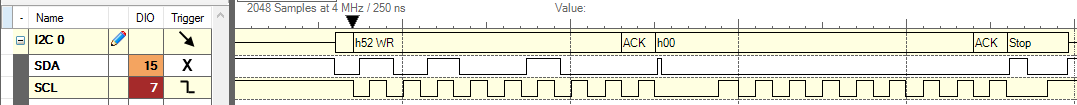
\includegraphics[width=\textwidth]{Test/images/writerequest}
	\caption{}
	\label{fig:NunchuckWriteValues}
\end{figure}

Det kan på figur \ref{fig:NunchuckWriteValues} ses at den første besked der måles er af typen "WR" (Write) til addressen 0x52 (Wii-Nunchuck I2C Slave Addressen). Hertil kommer et tilhørende \textit{ACK} (Acknowledge) fra Wii-Nunchuck. Til sidst sendes dataen Ox00 efterfulgt af at ACK fra Wii-Nunchuck. Til sidst afsluttes I2C transaktionen ved "Stop".

Det kan altså konkluderes at målingen er i overensstemmelse med forventningen om at en 0x00 byte skal sendes til Wii-Nunchuck for opstart af dataudveksling.

\textbf{Aflæsning af Wii-Nunchuck}

Efter vellykket afsendelse af 0x00 byten sker den egentlige aflæsning af Wii-Nunchuk input dataen.

Her forventes en række beskeder indeholdende 

På figur \ref{fig:NunchuckReadValues} ses I2C beskederne der bliver udvekslet mellem PSoC0 og Wii-Nunchuck efter vellykket Wii-Nunchuck Handshake. 

\begin{figure}[H]
	\centering
	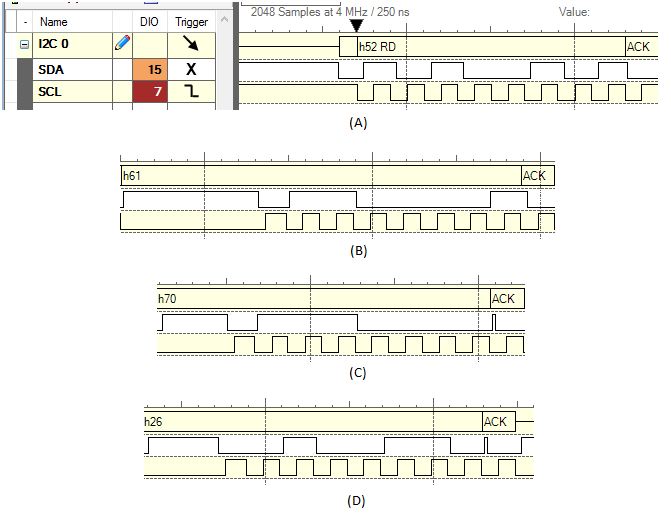
\includegraphics[width=\textwidth]{Test/images/readvaluesEdited.png}
	\caption{Tidslinje af aflæste I2C beskeder af PSoC0 fra Wii-Nunchuck}
	\label{fig:NunchuckReadValues}
\end{figure}

\subsubsection{I2C Protokol}

\subsection{Hardware}

\section{Integration}

\section{Accepttest}